% Created by tikzDevice version 0.10.1 on 2017-09-11 16:13:29
% !TEX encoding = UTF-8 Unicode
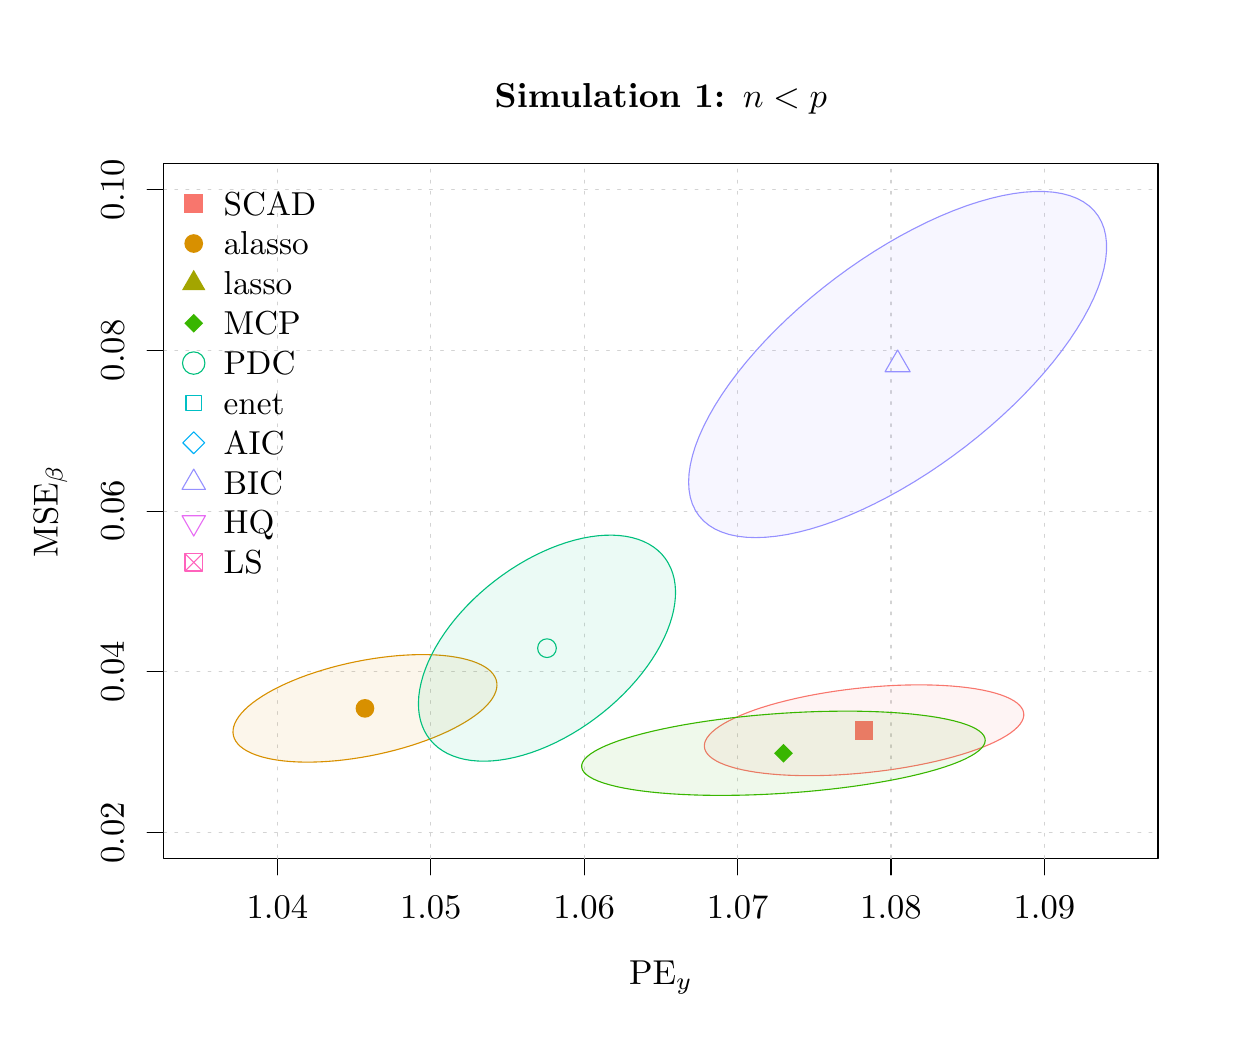
\begin{tikzpicture}[x=1pt,y=1pt]
\definecolor{fillColor}{RGB}{255,255,255}
\path[use as bounding box,fill=fillColor,fill opacity=0.00] (0,0) rectangle (433.62,361.35);
\begin{scope}
\path[clip] (  0.00,  0.00) rectangle (433.62,361.35);
\definecolor{drawColor}{RGB}{0,0,0}

\path[draw=drawColor,line width= 0.4pt,line join=round,line cap=round] ( 90.22, 61.20) -- (367.40, 61.20);

\path[draw=drawColor,line width= 0.4pt,line join=round,line cap=round] ( 90.22, 61.20) -- ( 90.22, 55.20);

\path[draw=drawColor,line width= 0.4pt,line join=round,line cap=round] (145.66, 61.20) -- (145.66, 55.20);

\path[draw=drawColor,line width= 0.4pt,line join=round,line cap=round] (201.09, 61.20) -- (201.09, 55.20);

\path[draw=drawColor,line width= 0.4pt,line join=round,line cap=round] (256.53, 61.20) -- (256.53, 55.20);

\path[draw=drawColor,line width= 0.4pt,line join=round,line cap=round] (311.96, 61.20) -- (311.96, 55.20);

\path[draw=drawColor,line width= 0.4pt,line join=round,line cap=round] (367.40, 61.20) -- (367.40, 55.20);

\node[text=drawColor,anchor=base,inner sep=0pt, outer sep=0pt, scale=  1.25] at ( 90.22, 39.60) {1.04};

\node[text=drawColor,anchor=base,inner sep=0pt, outer sep=0pt, scale=  1.25] at (145.66, 39.60) {1.05};

\node[text=drawColor,anchor=base,inner sep=0pt, outer sep=0pt, scale=  1.25] at (201.09, 39.60) {1.06};

\node[text=drawColor,anchor=base,inner sep=0pt, outer sep=0pt, scale=  1.25] at (256.53, 39.60) {1.07};

\node[text=drawColor,anchor=base,inner sep=0pt, outer sep=0pt, scale=  1.25] at (311.96, 39.60) {1.08};

\node[text=drawColor,anchor=base,inner sep=0pt, outer sep=0pt, scale=  1.25] at (367.40, 39.60) {1.09};

\path[draw=drawColor,line width= 0.4pt,line join=round,line cap=round] ( 49.20, 70.49) -- ( 49.20,302.86);

\path[draw=drawColor,line width= 0.4pt,line join=round,line cap=round] ( 49.20, 70.49) -- ( 43.20, 70.49);

\path[draw=drawColor,line width= 0.4pt,line join=round,line cap=round] ( 49.20,128.58) -- ( 43.20,128.58);

\path[draw=drawColor,line width= 0.4pt,line join=round,line cap=round] ( 49.20,186.67) -- ( 43.20,186.67);

\path[draw=drawColor,line width= 0.4pt,line join=round,line cap=round] ( 49.20,244.77) -- ( 43.20,244.77);

\path[draw=drawColor,line width= 0.4pt,line join=round,line cap=round] ( 49.20,302.86) -- ( 43.20,302.86);

\node[text=drawColor,rotate= 90.00,anchor=base,inner sep=0pt, outer sep=0pt, scale=  1.25] at ( 34.80, 70.49) {0.02};

\node[text=drawColor,rotate= 90.00,anchor=base,inner sep=0pt, outer sep=0pt, scale=  1.25] at ( 34.80,128.58) {0.04};

\node[text=drawColor,rotate= 90.00,anchor=base,inner sep=0pt, outer sep=0pt, scale=  1.25] at ( 34.80,186.67) {0.06};

\node[text=drawColor,rotate= 90.00,anchor=base,inner sep=0pt, outer sep=0pt, scale=  1.25] at ( 34.80,244.77) {0.08};

\node[text=drawColor,rotate= 90.00,anchor=base,inner sep=0pt, outer sep=0pt, scale=  1.25] at ( 34.80,302.86) {0.10};

\path[draw=drawColor,line width= 0.4pt,line join=round,line cap=round] ( 49.20, 61.20) --
	(408.42, 61.20) --
	(408.42,312.15) --
	( 49.20,312.15) --
	( 49.20, 61.20);
\end{scope}
\begin{scope}
\path[clip] (  0.00,  0.00) rectangle (433.62,361.35);
\definecolor{drawColor}{RGB}{0,0,0}

\node[text=drawColor,anchor=base,inner sep=0pt, outer sep=0pt, scale=  1.25] at (228.81,332.44) {\bfseries Simulation 1: $n < p$};

\node[text=drawColor,anchor=base,inner sep=0pt, outer sep=0pt, scale=  1.25] at (228.81, 15.60) {PE$_{y}$};

\node[text=drawColor,rotate= 90.00,anchor=base,inner sep=0pt, outer sep=0pt, scale=  1.25] at ( 10.80,186.67) {MSE$_{\beta}$};
\end{scope}
\begin{scope}
\path[clip] ( 49.20, 61.20) rectangle (408.42,312.15);
\definecolor{drawColor}{RGB}{211,211,211}

\path[draw=drawColor,line width= 0.4pt,dash pattern=on 1pt off 3pt ,line join=round,line cap=round] ( 90.22, 61.20) -- ( 90.22,312.15);

\path[draw=drawColor,line width= 0.4pt,dash pattern=on 1pt off 3pt ,line join=round,line cap=round] (145.66, 61.20) -- (145.66,312.15);

\path[draw=drawColor,line width= 0.4pt,dash pattern=on 1pt off 3pt ,line join=round,line cap=round] (201.09, 61.20) -- (201.09,312.15);

\path[draw=drawColor,line width= 0.4pt,dash pattern=on 1pt off 3pt ,line join=round,line cap=round] (256.53, 61.20) -- (256.53,312.15);

\path[draw=drawColor,line width= 0.4pt,dash pattern=on 1pt off 3pt ,line join=round,line cap=round] (311.96, 61.20) -- (311.96,312.15);

\path[draw=drawColor,line width= 0.4pt,dash pattern=on 1pt off 3pt ,line join=round,line cap=round] (367.40, 61.20) -- (367.40,312.15);

\path[draw=drawColor,line width= 0.4pt,dash pattern=on 1pt off 3pt ,line join=round,line cap=round] ( 49.20, 70.49) -- (408.42, 70.49);

\path[draw=drawColor,line width= 0.4pt,dash pattern=on 1pt off 3pt ,line join=round,line cap=round] ( 49.20,128.58) -- (408.42,128.58);

\path[draw=drawColor,line width= 0.4pt,dash pattern=on 1pt off 3pt ,line join=round,line cap=round] ( 49.20,186.67) -- (408.42,186.67);

\path[draw=drawColor,line width= 0.4pt,dash pattern=on 1pt off 3pt ,line join=round,line cap=round] ( 49.20,244.77) -- (408.42,244.77);

\path[draw=drawColor,line width= 0.4pt,dash pattern=on 1pt off 3pt ,line join=round,line cap=round] ( 49.20,302.86) -- (408.42,302.86);
\definecolor{fillColor}{RGB}{248,118,109}

\path[fill=fillColor] (298.85,104.09) --
	(305.60,104.09) --
	(305.60,110.84) --
	(298.85,110.84) --
	cycle;
\definecolor{drawColor}{RGB}{248,118,109}

\path[draw=drawColor,line width= 0.4pt,line join=round,line cap=round] (349.55,120.92) --
	(347.36,121.49) --
	(344.99,122.00) --
	(342.45,122.46) --
	(339.74,122.85) --
	(336.88,123.18) --
	(333.88,123.45) --
	(330.76,123.65) --
	(327.52,123.79) --
	(324.18,123.86) --
	(320.75,123.87) --
	(317.24,123.81) --
	(313.68,123.69) --
	(310.07,123.50) --
	(306.43,123.24) --
	(302.77,122.92) --
	(299.10,122.54) --
	(295.46,122.10) --
	(291.83,121.60) --
	(288.25,121.04) --
	(284.73,120.43) --
	(281.28,119.77) --
	(277.91,119.05) --
	(274.64,118.29) --
	(271.48,117.49) --
	(268.44,116.65) --
	(265.54,115.76) --
	(262.79,114.85) --
	(260.20,113.90) --
	(257.77,112.93) --
	(255.53,111.94) --
	(253.47,110.93) --
	(251.61,109.91) --
	(249.95,108.87) --
	(248.50,107.83) --
	(247.27,106.79) --
	(246.27,105.75) --
	(245.48,104.72) --
	(244.93,103.70) --
	(244.60,102.70) --
	(244.51,101.71) --
	(244.65,100.75) --
	(245.02, 99.81) --
	(245.63, 98.91) --
	(246.46, 98.03) --
	(247.51, 97.20) --
	(248.79, 96.41) --
	(250.28, 95.66) --
	(251.98, 94.96) --
	(253.88, 94.32) --
	(255.97, 93.72) --
	(258.26, 93.18) --
	(260.72, 92.70) --
	(263.34, 92.27) --
	(266.13, 91.91) --
	(269.06, 91.61) --
	(272.12, 91.37) --
	(275.30, 91.20) --
	(278.60, 91.10) --
	(281.98, 91.06) --
	(285.45, 91.08) --
	(288.99, 91.17) --
	(292.58, 91.33) --
	(296.21, 91.56) --
	(299.86, 91.84) --
	(303.52, 92.19) --
	(307.18, 92.60) --
	(310.82, 93.07) --
	(314.42, 93.60) --
	(317.97, 94.19) --
	(321.46, 94.83) --
	(324.88, 95.52) --
	(328.20, 96.25) --
	(331.41, 97.04) --
	(334.51, 97.86) --
	(337.48, 98.72) --
	(340.31, 99.62) --
	(342.98,100.55) --
	(345.49,101.51) --
	(347.83,102.49) --
	(349.98,103.49) --
	(351.94,104.51) --
	(353.70,105.54) --
	(355.26,106.58) --
	(356.59,107.62) --
	(357.71,108.66) --
	(358.61,109.69) --
	(359.28,110.72) --
	(359.72,111.74) --
	(359.93,112.73) --
	(359.90,113.71) --
	(359.65,114.66) --
	(359.16,115.58) --
	(358.44,116.47) --
	(357.50,117.32) --
	(356.34,118.13) --
	(354.95,118.90) --
	(353.36,119.62) --
	(351.55,120.30) --
	(349.55,120.92);
\definecolor{fillColor}{RGB}{248,118,109}

\path[fill=fillColor,fill opacity=0.08] (349.55,120.92) --
	(347.36,121.49) --
	(344.99,122.00) --
	(342.45,122.46) --
	(339.74,122.85) --
	(336.88,123.18) --
	(333.88,123.45) --
	(330.76,123.65) --
	(327.52,123.79) --
	(324.18,123.86) --
	(320.75,123.87) --
	(317.24,123.81) --
	(313.68,123.69) --
	(310.07,123.50) --
	(306.43,123.24) --
	(302.77,122.92) --
	(299.10,122.54) --
	(295.46,122.10) --
	(291.83,121.60) --
	(288.25,121.04) --
	(284.73,120.43) --
	(281.28,119.77) --
	(277.91,119.05) --
	(274.64,118.29) --
	(271.48,117.49) --
	(268.44,116.65) --
	(265.54,115.76) --
	(262.79,114.85) --
	(260.20,113.90) --
	(257.77,112.93) --
	(255.53,111.94) --
	(253.47,110.93) --
	(251.61,109.91) --
	(249.95,108.87) --
	(248.50,107.83) --
	(247.27,106.79) --
	(246.27,105.75) --
	(245.48,104.72) --
	(244.93,103.70) --
	(244.60,102.70) --
	(244.51,101.71) --
	(244.65,100.75) --
	(245.02, 99.81) --
	(245.63, 98.91) --
	(246.46, 98.03) --
	(247.51, 97.20) --
	(248.79, 96.41) --
	(250.28, 95.66) --
	(251.98, 94.96) --
	(253.88, 94.32) --
	(255.97, 93.72) --
	(258.26, 93.18) --
	(260.72, 92.70) --
	(263.34, 92.27) --
	(266.13, 91.91) --
	(269.06, 91.61) --
	(272.12, 91.37) --
	(275.30, 91.20) --
	(278.60, 91.10) --
	(281.98, 91.06) --
	(285.45, 91.08) --
	(288.99, 91.17) --
	(292.58, 91.33) --
	(296.21, 91.56) --
	(299.86, 91.84) --
	(303.52, 92.19) --
	(307.18, 92.60) --
	(310.82, 93.07) --
	(314.42, 93.60) --
	(317.97, 94.19) --
	(321.46, 94.83) --
	(324.88, 95.52) --
	(328.20, 96.25) --
	(331.41, 97.04) --
	(334.51, 97.86) --
	(337.48, 98.72) --
	(340.31, 99.62) --
	(342.98,100.55) --
	(345.49,101.51) --
	(347.83,102.49) --
	(349.98,103.49) --
	(351.94,104.51) --
	(353.70,105.54) --
	(355.26,106.58) --
	(356.59,107.62) --
	(357.71,108.66) --
	(358.61,109.69) --
	(359.28,110.72) --
	(359.72,111.74) --
	(359.93,112.73) --
	(359.90,113.71) --
	(359.65,114.66) --
	(359.16,115.58) --
	(358.44,116.47) --
	(357.50,117.32) --
	(356.34,118.13) --
	(354.95,118.90) --
	(353.36,119.62) --
	(351.55,120.30) --
	(349.55,120.92) --
	cycle;
\definecolor{fillColor}{RGB}{216,144,0}

\path[fill=fillColor] (121.88,115.38) circle (  3.38);
\definecolor{drawColor}{RGB}{216,144,0}

\path[draw=drawColor,line width= 0.4pt,line join=round,line cap=round] (162.28,131.84) --
	(160.60,132.46) --
	(158.75,133.01) --
	(156.76,133.50) --
	(154.62,133.90) --
	(152.36,134.24) --
	(149.97,134.50) --
	(147.47,134.68) --
	(144.87,134.78) --
	(142.17,134.81) --
	(139.39,134.76) --
	(136.54,134.62) --
	(133.63,134.42) --
	(130.68,134.13) --
	(127.69,133.77) --
	(124.67,133.34) --
	(121.65,132.83) --
	(118.62,132.25) --
	(115.61,131.61) --
	(112.63,130.90) --
	(109.68,130.13) --
	(106.78,129.29) --
	(103.94,128.41) --
	(101.17,127.47) --
	( 98.49,126.48) --
	( 95.90,125.44) --
	( 93.42,124.37) --
	( 91.05,123.26) --
	( 88.80,122.12) --
	( 86.69,120.95) --
	( 84.72,119.75) --
	( 82.90,118.54) --
	( 81.23,117.32) --
	( 79.73,116.09) --
	( 78.40,114.86) --
	( 77.25,113.63) --
	( 76.27,112.40) --
	( 75.48,111.19) --
	( 74.87,110.00) --
	( 74.46,108.82) --
	( 74.23,107.68) --
	( 74.20,106.56) --
	( 74.36,105.48) --
	( 74.71,104.44) --
	( 75.25,103.44) --
	( 75.98,102.50) --
	( 76.89,101.60) --
	( 77.98,100.76) --
	( 79.26, 99.98) --
	( 80.70, 99.26) --
	( 82.31, 98.60) --
	( 84.07, 98.01) --
	( 85.99, 97.50) --
	( 88.06, 97.05) --
	( 90.26, 96.68) --
	( 92.59, 96.38) --
	( 95.03, 96.16) --
	( 97.59, 96.02) --
	(100.24, 95.95) --
	(102.98, 95.97) --
	(105.79, 96.06) --
	(108.67, 96.23) --
	(111.61, 96.47) --
	(114.58, 96.80) --
	(117.59, 97.20) --
	(120.61, 97.67) --
	(123.63, 98.21) --
	(126.65, 98.82) --
	(129.65, 99.50) --
	(132.62,100.24) --
	(135.55,101.04) --
	(138.42,101.90) --
	(141.22,102.82) --
	(143.95,103.78) --
	(146.59,104.79) --
	(149.12,105.85) --
	(151.55,106.94) --
	(153.86,108.07) --
	(156.04,109.23) --
	(158.08,110.41) --
	(159.98,111.61) --
	(161.72,112.82) --
	(163.31,114.05) --
	(164.72,115.28) --
	(165.96,116.52) --
	(167.03,117.74) --
	(167.92,118.96) --
	(168.61,120.17) --
	(169.12,121.35) --
	(169.45,122.51) --
	(169.57,123.64) --
	(169.51,124.74) --
	(169.26,125.80) --
	(168.81,126.82) --
	(168.18,127.79) --
	(167.36,128.72) --
	(166.35,129.59) --
	(165.17,130.40) --
	(163.81,131.15) --
	(162.28,131.84);
\definecolor{fillColor}{RGB}{216,144,0}

\path[fill=fillColor,fill opacity=0.08] (162.28,131.84) --
	(160.60,132.46) --
	(158.75,133.01) --
	(156.76,133.50) --
	(154.62,133.90) --
	(152.36,134.24) --
	(149.97,134.50) --
	(147.47,134.68) --
	(144.87,134.78) --
	(142.17,134.81) --
	(139.39,134.76) --
	(136.54,134.62) --
	(133.63,134.42) --
	(130.68,134.13) --
	(127.69,133.77) --
	(124.67,133.34) --
	(121.65,132.83) --
	(118.62,132.25) --
	(115.61,131.61) --
	(112.63,130.90) --
	(109.68,130.13) --
	(106.78,129.29) --
	(103.94,128.41) --
	(101.17,127.47) --
	( 98.49,126.48) --
	( 95.90,125.44) --
	( 93.42,124.37) --
	( 91.05,123.26) --
	( 88.80,122.12) --
	( 86.69,120.95) --
	( 84.72,119.75) --
	( 82.90,118.54) --
	( 81.23,117.32) --
	( 79.73,116.09) --
	( 78.40,114.86) --
	( 77.25,113.63) --
	( 76.27,112.40) --
	( 75.48,111.19) --
	( 74.87,110.00) --
	( 74.46,108.82) --
	( 74.23,107.68) --
	( 74.20,106.56) --
	( 74.36,105.48) --
	( 74.71,104.44) --
	( 75.25,103.44) --
	( 75.98,102.50) --
	( 76.89,101.60) --
	( 77.98,100.76) --
	( 79.26, 99.98) --
	( 80.70, 99.26) --
	( 82.31, 98.60) --
	( 84.07, 98.01) --
	( 85.99, 97.50) --
	( 88.06, 97.05) --
	( 90.26, 96.68) --
	( 92.59, 96.38) --
	( 95.03, 96.16) --
	( 97.59, 96.02) --
	(100.24, 95.95) --
	(102.98, 95.97) --
	(105.79, 96.06) --
	(108.67, 96.23) --
	(111.61, 96.47) --
	(114.58, 96.80) --
	(117.59, 97.20) --
	(120.61, 97.67) --
	(123.63, 98.21) --
	(126.65, 98.82) --
	(129.65, 99.50) --
	(132.62,100.24) --
	(135.55,101.04) --
	(138.42,101.90) --
	(141.22,102.82) --
	(143.95,103.78) --
	(146.59,104.79) --
	(149.12,105.85) --
	(151.55,106.94) --
	(153.86,108.07) --
	(156.04,109.23) --
	(158.08,110.41) --
	(159.98,111.61) --
	(161.72,112.82) --
	(163.31,114.05) --
	(164.72,115.28) --
	(165.96,116.52) --
	(167.03,117.74) --
	(167.92,118.96) --
	(168.61,120.17) --
	(169.12,121.35) --
	(169.45,122.51) --
	(169.57,123.64) --
	(169.51,124.74) --
	(169.26,125.80) --
	(168.81,126.82) --
	(168.18,127.79) --
	(167.36,128.72) --
	(166.35,129.59) --
	(165.17,130.40) --
	(163.81,131.15) --
	(162.28,131.84) --
	cycle;
\definecolor{fillColor}{RGB}{57,182,0}

\path[fill=fillColor] (269.72, 99.16) --
	(273.09,102.53) --
	(276.47, 99.16) --
	(273.09, 95.78) --
	cycle;
\definecolor{drawColor}{RGB}{57,182,0}

\path[draw=drawColor,line width= 0.4pt,line join=round,line cap=round] (332.08,111.47) --
	(329.24,112.02) --
	(326.18,112.51) --
	(322.90,112.94) --
	(319.42,113.33) --
	(315.76,113.65) --
	(311.92,113.92) --
	(307.93,114.12) --
	(303.80,114.27) --
	(299.54,114.36) --
	(295.18,114.38) --
	(290.73,114.34) --
	(286.20,114.25) --
	(281.63,114.09) --
	(277.02,113.87) --
	(272.39,113.59) --
	(267.77,113.25) --
	(263.17,112.86) --
	(258.60,112.41) --
	(254.10,111.91) --
	(249.67,111.36) --
	(245.34,110.76) --
	(241.12,110.11) --
	(237.03,109.42) --
	(233.08,108.68) --
	(229.30,107.91) --
	(225.69,107.10) --
	(222.27,106.26) --
	(219.05,105.39) --
	(216.06,104.50) --
	(213.29,103.59) --
	(210.76,102.65) --
	(208.49,101.71) --
	(206.47,100.75) --
	(204.73, 99.79) --
	(203.26, 98.82) --
	(202.07, 97.86) --
	(201.16, 96.90) --
	(200.55, 95.95) --
	(200.23, 95.01) --
	(200.20, 94.09) --
	(200.46, 93.19) --
	(201.02, 92.31) --
	(201.87, 91.46) --
	(203.00, 90.65) --
	(204.42, 89.86) --
	(206.11, 89.12) --
	(208.07, 88.41) --
	(210.30, 87.75) --
	(212.77, 87.13) --
	(215.49, 86.56) --
	(218.44, 86.05) --
	(221.62, 85.58) --
	(225.00, 85.17) --
	(228.57, 84.82) --
	(232.32, 84.52) --
	(236.24, 84.29) --
	(240.30, 84.11) --
	(244.50, 83.99) --
	(248.81, 83.94) --
	(253.22, 83.95) --
	(257.71, 84.01) --
	(262.26, 84.14) --
	(266.86, 84.33) --
	(271.48, 84.58) --
	(276.10, 84.89) --
	(280.72, 85.25) --
	(285.30, 85.67) --
	(289.84, 86.15) --
	(294.30, 86.67) --
	(298.69, 87.25) --
	(302.97, 87.88) --
	(307.12, 88.55) --
	(311.15, 89.26) --
	(315.01, 90.01) --
	(318.71, 90.80) --
	(322.23, 91.63) --
	(325.55, 92.48) --
	(328.65, 93.36) --
	(331.54, 94.27) --
	(334.18, 95.19) --
	(336.59, 96.13) --
	(338.73, 97.09) --
	(340.61, 98.05) --
	(342.22, 99.01) --
	(343.56, 99.98) --
	(344.60,100.94) --
	(345.36,101.89) --
	(345.83,102.84) --
	(346.01,103.77) --
	(345.89,104.68) --
	(345.48,105.57) --
	(344.78,106.43) --
	(343.78,107.26) --
	(342.51,108.07) --
	(340.95,108.83) --
	(339.12,109.56) --
	(337.03,110.24) --
	(334.68,110.88) --
	(332.08,111.47);
\definecolor{fillColor}{RGB}{57,182,0}

\path[fill=fillColor,fill opacity=0.08] (332.08,111.47) --
	(329.24,112.02) --
	(326.18,112.51) --
	(322.90,112.94) --
	(319.42,113.33) --
	(315.76,113.65) --
	(311.92,113.92) --
	(307.93,114.12) --
	(303.80,114.27) --
	(299.54,114.36) --
	(295.18,114.38) --
	(290.73,114.34) --
	(286.20,114.25) --
	(281.63,114.09) --
	(277.02,113.87) --
	(272.39,113.59) --
	(267.77,113.25) --
	(263.17,112.86) --
	(258.60,112.41) --
	(254.10,111.91) --
	(249.67,111.36) --
	(245.34,110.76) --
	(241.12,110.11) --
	(237.03,109.42) --
	(233.08,108.68) --
	(229.30,107.91) --
	(225.69,107.10) --
	(222.27,106.26) --
	(219.05,105.39) --
	(216.06,104.50) --
	(213.29,103.59) --
	(210.76,102.65) --
	(208.49,101.71) --
	(206.47,100.75) --
	(204.73, 99.79) --
	(203.26, 98.82) --
	(202.07, 97.86) --
	(201.16, 96.90) --
	(200.55, 95.95) --
	(200.23, 95.01) --
	(200.20, 94.09) --
	(200.46, 93.19) --
	(201.02, 92.31) --
	(201.87, 91.46) --
	(203.00, 90.65) --
	(204.42, 89.86) --
	(206.11, 89.12) --
	(208.07, 88.41) --
	(210.30, 87.75) --
	(212.77, 87.13) --
	(215.49, 86.56) --
	(218.44, 86.05) --
	(221.62, 85.58) --
	(225.00, 85.17) --
	(228.57, 84.82) --
	(232.32, 84.52) --
	(236.24, 84.29) --
	(240.30, 84.11) --
	(244.50, 83.99) --
	(248.81, 83.94) --
	(253.22, 83.95) --
	(257.71, 84.01) --
	(262.26, 84.14) --
	(266.86, 84.33) --
	(271.48, 84.58) --
	(276.10, 84.89) --
	(280.72, 85.25) --
	(285.30, 85.67) --
	(289.84, 86.15) --
	(294.30, 86.67) --
	(298.69, 87.25) --
	(302.97, 87.88) --
	(307.12, 88.55) --
	(311.15, 89.26) --
	(315.01, 90.01) --
	(318.71, 90.80) --
	(322.23, 91.63) --
	(325.55, 92.48) --
	(328.65, 93.36) --
	(331.54, 94.27) --
	(334.18, 95.19) --
	(336.59, 96.13) --
	(338.73, 97.09) --
	(340.61, 98.05) --
	(342.22, 99.01) --
	(343.56, 99.98) --
	(344.60,100.94) --
	(345.36,101.89) --
	(345.83,102.84) --
	(346.01,103.77) --
	(345.89,104.68) --
	(345.48,105.57) --
	(344.78,106.43) --
	(343.78,107.26) --
	(342.51,108.07) --
	(340.95,108.83) --
	(339.12,109.56) --
	(337.03,110.24) --
	(334.68,110.88) --
	(332.08,111.47) --
	cycle;
\definecolor{drawColor}{RGB}{0,191,125}

\path[draw=drawColor,line width= 0.4pt,line join=round,line cap=round] (187.65,137.13) circle (  3.38);

\path[draw=drawColor,line width= 0.4pt,line join=round,line cap=round] (227.77,172.42) --
	(226.21,173.65) --
	(224.49,174.74) --
	(222.62,175.67) --
	(220.61,176.45) --
	(218.47,177.07) --
	(216.20,177.54) --
	(213.82,177.83) --
	(211.33,177.97) --
	(208.75,177.94) --
	(206.09,177.75) --
	(203.34,177.39) --
	(200.54,176.87) --
	(197.68,176.19) --
	(194.79,175.35) --
	(191.86,174.36) --
	(188.92,173.22) --
	(185.97,171.93) --
	(183.03,170.51) --
	(180.11,168.95) --
	(177.22,167.26) --
	(174.37,165.45) --
	(171.57,163.52) --
	(168.84,161.49) --
	(166.19,159.37) --
	(163.62,157.15) --
	(161.14,154.85) --
	(158.78,152.48) --
	(156.53,150.05) --
	(154.40,147.57) --
	(152.41,145.04) --
	(150.57,142.48) --
	(148.87,139.90) --
	(147.32,137.31) --
	(145.94,134.72) --
	(144.73,132.14) --
	(143.69,129.58) --
	(142.83,127.05) --
	(142.15,124.56) --
	(141.65,122.12) --
	(141.33,119.74) --
	(141.21,117.43) --
	(141.26,115.20) --
	(141.51,113.06) --
	(141.94,111.02) --
	(142.56,109.08) --
	(143.36,107.25) --
	(144.33,105.55) --
	(145.48,103.97) --
	(146.81,102.52) --
	(148.29,101.22) --
	(149.93,100.06) --
	(151.73, 99.04) --
	(153.67, 98.19) --
	(155.75, 97.48) --
	(157.95, 96.94) --
	(160.28, 96.56) --
	(162.71, 96.35) --
	(165.25, 96.29) --
	(167.87, 96.40) --
	(170.58, 96.68) --
	(173.35, 97.12) --
	(176.18, 97.72) --
	(179.06, 98.48) --
	(181.97, 99.39) --
	(184.91,100.46) --
	(187.85,101.67) --
	(190.80,103.03) --
	(193.73,104.52) --
	(196.64,106.15) --
	(199.51,107.90) --
	(202.34,109.77) --
	(205.10,111.75) --
	(207.80,113.83) --
	(210.41,116.00) --
	(212.93,118.26) --
	(215.35,120.59) --
	(217.66,123.00) --
	(219.85,125.45) --
	(221.91,127.96) --
	(223.83,130.50) --
	(225.60,133.07) --
	(227.23,135.66) --
	(228.69,138.25) --
	(229.99,140.84) --
	(231.11,143.41) --
	(232.06,145.96) --
	(232.84,148.47) --
	(233.43,150.93) --
	(233.83,153.34) --
	(234.06,155.69) --
	(234.09,157.96) --
	(233.94,160.15) --
	(233.60,162.24) --
	(233.07,164.23) --
	(232.36,166.12) --
	(231.48,167.88) --
	(230.41,169.53) --
	(229.18,171.04) --
	(227.77,172.42);
\definecolor{fillColor}{RGB}{0,191,125}

\path[fill=fillColor,fill opacity=0.08] (227.77,172.42) --
	(226.21,173.65) --
	(224.49,174.74) --
	(222.62,175.67) --
	(220.61,176.45) --
	(218.47,177.07) --
	(216.20,177.54) --
	(213.82,177.83) --
	(211.33,177.97) --
	(208.75,177.94) --
	(206.09,177.75) --
	(203.34,177.39) --
	(200.54,176.87) --
	(197.68,176.19) --
	(194.79,175.35) --
	(191.86,174.36) --
	(188.92,173.22) --
	(185.97,171.93) --
	(183.03,170.51) --
	(180.11,168.95) --
	(177.22,167.26) --
	(174.37,165.45) --
	(171.57,163.52) --
	(168.84,161.49) --
	(166.19,159.37) --
	(163.62,157.15) --
	(161.14,154.85) --
	(158.78,152.48) --
	(156.53,150.05) --
	(154.40,147.57) --
	(152.41,145.04) --
	(150.57,142.48) --
	(148.87,139.90) --
	(147.32,137.31) --
	(145.94,134.72) --
	(144.73,132.14) --
	(143.69,129.58) --
	(142.83,127.05) --
	(142.15,124.56) --
	(141.65,122.12) --
	(141.33,119.74) --
	(141.21,117.43) --
	(141.26,115.20) --
	(141.51,113.06) --
	(141.94,111.02) --
	(142.56,109.08) --
	(143.36,107.25) --
	(144.33,105.55) --
	(145.48,103.97) --
	(146.81,102.52) --
	(148.29,101.22) --
	(149.93,100.06) --
	(151.73, 99.04) --
	(153.67, 98.19) --
	(155.75, 97.48) --
	(157.95, 96.94) --
	(160.28, 96.56) --
	(162.71, 96.35) --
	(165.25, 96.29) --
	(167.87, 96.40) --
	(170.58, 96.68) --
	(173.35, 97.12) --
	(176.18, 97.72) --
	(179.06, 98.48) --
	(181.97, 99.39) --
	(184.91,100.46) --
	(187.85,101.67) --
	(190.80,103.03) --
	(193.73,104.52) --
	(196.64,106.15) --
	(199.51,107.90) --
	(202.34,109.77) --
	(205.10,111.75) --
	(207.80,113.83) --
	(210.41,116.00) --
	(212.93,118.26) --
	(215.35,120.59) --
	(217.66,123.00) --
	(219.85,125.45) --
	(221.91,127.96) --
	(223.83,130.50) --
	(225.60,133.07) --
	(227.23,135.66) --
	(228.69,138.25) --
	(229.99,140.84) --
	(231.11,143.41) --
	(232.06,145.96) --
	(232.84,148.47) --
	(233.43,150.93) --
	(233.83,153.34) --
	(234.06,155.69) --
	(234.09,157.96) --
	(233.94,160.15) --
	(233.60,162.24) --
	(233.07,164.23) --
	(232.36,166.12) --
	(231.48,167.88) --
	(230.41,169.53) --
	(229.18,171.04) --
	(227.77,172.42) --
	cycle;
\definecolor{drawColor}{RGB}{149,144,255}

\path[draw=drawColor,line width= 0.4pt,line join=round,line cap=round] (314.35,244.88) --
	(318.89,237.01) --
	(309.80,237.01) --
	(314.35,244.88);

\path[draw=drawColor,line width= 0.4pt,line join=round,line cap=round] (383.55,296.95) --
	(381.49,298.42) --
	(379.16,299.66) --
	(376.57,300.65) --
	(373.73,301.40) --
	(370.66,301.90) --
	(367.35,302.15) --
	(363.83,302.15) --
	(360.11,301.90) --
	(356.21,301.39) --
	(352.14,300.64) --
	(347.92,299.64) --
	(343.56,298.40) --
	(339.08,296.93) --
	(334.51,295.22) --
	(329.85,293.29) --
	(325.13,291.14) --
	(320.37,288.78) --
	(315.58,286.23) --
	(310.79,283.49) --
	(306.01,280.57) --
	(301.27,277.49) --
	(296.58,274.26) --
	(291.96,270.88) --
	(287.43,267.38) --
	(283.01,263.77) --
	(278.71,260.06) --
	(274.56,256.27) --
	(270.57,252.42) --
	(266.75,248.51) --
	(263.13,244.56) --
	(259.71,240.60) --
	(256.52,236.63) --
	(253.55,232.67) --
	(250.83,228.74) --
	(248.37,224.86) --
	(246.17,221.03) --
	(244.25,217.28) --
	(242.61,213.62) --
	(241.25,210.07) --
	(240.20,206.63) --
	(239.44,203.32) --
	(238.98,200.17) --
	(238.83,197.17) --
	(238.98,194.34) --
	(239.43,191.70) --
	(240.18,189.24) --
	(241.24,186.99) --
	(242.59,184.96) --
	(244.22,183.14) --
	(246.14,181.55) --
	(248.34,180.19) --
	(250.80,179.08) --
	(253.51,178.20) --
	(256.47,177.58) --
	(259.67,177.20) --
	(263.08,177.08) --
	(266.70,177.21) --
	(270.51,177.59) --
	(274.50,178.21) --
	(278.65,179.09) --
	(282.94,180.21) --
	(287.36,181.57) --
	(291.89,183.16) --
	(296.51,184.98) --
	(301.20,187.02) --
	(305.94,189.28) --
	(310.72,191.73) --
	(315.51,194.38) --
	(320.30,197.21) --
	(325.06,200.21) --
	(329.78,203.37) --
	(334.44,206.68) --
	(339.02,210.11) --
	(343.49,213.67) --
	(347.85,217.33) --
	(352.08,221.09) --
	(356.15,224.91) --
	(360.06,228.80) --
	(363.78,232.73) --
	(367.30,236.68) --
	(370.61,240.65) --
	(373.69,244.62) --
	(376.54,248.56) --
	(379.13,252.47) --
	(381.46,256.33) --
	(383.52,260.12) --
	(385.30,263.82) --
	(386.80,267.43) --
	(388.01,270.93) --
	(388.92,274.30) --
	(389.53,277.54) --
	(389.83,280.62) --
	(389.83,283.53) --
	(389.53,286.27) --
	(388.93,288.82) --
	(388.02,291.17) --
	(386.82,293.32) --
	(385.33,295.24) --
	(383.55,296.95);
\definecolor{fillColor}{RGB}{149,144,255}

\path[fill=fillColor,fill opacity=0.08] (383.55,296.95) --
	(381.49,298.42) --
	(379.16,299.66) --
	(376.57,300.65) --
	(373.73,301.40) --
	(370.66,301.90) --
	(367.35,302.15) --
	(363.83,302.15) --
	(360.11,301.90) --
	(356.21,301.39) --
	(352.14,300.64) --
	(347.92,299.64) --
	(343.56,298.40) --
	(339.08,296.93) --
	(334.51,295.22) --
	(329.85,293.29) --
	(325.13,291.14) --
	(320.37,288.78) --
	(315.58,286.23) --
	(310.79,283.49) --
	(306.01,280.57) --
	(301.27,277.49) --
	(296.58,274.26) --
	(291.96,270.88) --
	(287.43,267.38) --
	(283.01,263.77) --
	(278.71,260.06) --
	(274.56,256.27) --
	(270.57,252.42) --
	(266.75,248.51) --
	(263.13,244.56) --
	(259.71,240.60) --
	(256.52,236.63) --
	(253.55,232.67) --
	(250.83,228.74) --
	(248.37,224.86) --
	(246.17,221.03) --
	(244.25,217.28) --
	(242.61,213.62) --
	(241.25,210.07) --
	(240.20,206.63) --
	(239.44,203.32) --
	(238.98,200.17) --
	(238.83,197.17) --
	(238.98,194.34) --
	(239.43,191.70) --
	(240.18,189.24) --
	(241.24,186.99) --
	(242.59,184.96) --
	(244.22,183.14) --
	(246.14,181.55) --
	(248.34,180.19) --
	(250.80,179.08) --
	(253.51,178.20) --
	(256.47,177.58) --
	(259.67,177.20) --
	(263.08,177.08) --
	(266.70,177.21) --
	(270.51,177.59) --
	(274.50,178.21) --
	(278.65,179.09) --
	(282.94,180.21) --
	(287.36,181.57) --
	(291.89,183.16) --
	(296.51,184.98) --
	(301.20,187.02) --
	(305.94,189.28) --
	(310.72,191.73) --
	(315.51,194.38) --
	(320.30,197.21) --
	(325.06,200.21) --
	(329.78,203.37) --
	(334.44,206.68) --
	(339.02,210.11) --
	(343.49,213.67) --
	(347.85,217.33) --
	(352.08,221.09) --
	(356.15,224.91) --
	(360.06,228.80) --
	(363.78,232.73) --
	(367.30,236.68) --
	(370.61,240.65) --
	(373.69,244.62) --
	(376.54,248.56) --
	(379.13,252.47) --
	(381.46,256.33) --
	(383.52,260.12) --
	(385.30,263.82) --
	(386.80,267.43) --
	(388.01,270.93) --
	(388.92,274.30) --
	(389.53,277.54) --
	(389.83,280.62) --
	(389.83,283.53) --
	(389.53,286.27) --
	(388.93,288.82) --
	(388.02,291.17) --
	(386.82,293.32) --
	(385.33,295.24) --
	(383.55,296.95) --
	cycle;
\definecolor{fillColor}{RGB}{248,118,109}

\path[fill=fillColor] ( 56.63,294.38) --
	( 63.38,294.38) --
	( 63.38,301.12) --
	( 56.63,301.12) --
	cycle;
\definecolor{fillColor}{RGB}{216,144,0}

\path[fill=fillColor] ( 60.00,283.35) circle (  3.38);
\definecolor{fillColor}{RGB}{163,165,0}

\path[fill=fillColor] ( 60.00,273.85) --
	( 64.24,266.50) --
	( 55.76,266.50) --
	cycle;
\definecolor{fillColor}{RGB}{57,182,0}

\path[fill=fillColor] ( 56.63,254.55) --
	( 60.00,257.93) --
	( 63.38,254.55) --
	( 60.00,251.18) --
	cycle;
\definecolor{drawColor}{RGB}{0,191,125}

\path[draw=drawColor,line width= 0.4pt,line join=round,line cap=round] ( 60.00,240.15) circle (  4.05);
\definecolor{drawColor}{RGB}{0,191,196}

\path[draw=drawColor,line width= 0.4pt,line join=round,line cap=round] ( 57.21,222.96) rectangle ( 62.79,228.54);
\definecolor{drawColor}{RGB}{0,176,246}

\path[draw=drawColor,line width= 0.4pt,line join=round,line cap=round] ( 60.00,207.40) --
	( 63.95,211.35) --
	( 60.00,215.30) --
	( 56.05,211.35) --
	( 60.00,207.40);
\definecolor{drawColor}{RGB}{149,144,255}

\path[draw=drawColor,line width= 0.4pt,line join=round,line cap=round] ( 60.00,201.85) --
	( 64.24,194.50) --
	( 55.76,194.50) --
	( 60.00,201.85);
\definecolor{drawColor}{RGB}{231,107,243}

\path[draw=drawColor,line width= 0.4pt,line join=round,line cap=round] ( 60.00,177.65) --
	( 64.24,185.00) --
	( 55.76,185.00) --
	( 60.00,177.65);
\definecolor{drawColor}{RGB}{255,98,188}

\path[draw=drawColor,line width= 0.4pt,line join=round,line cap=round] ( 56.85,165.00) rectangle ( 63.15,171.30);

\path[draw=drawColor,line width= 0.4pt,line join=round,line cap=round] ( 56.85,165.00) -- ( 63.15,171.30);

\path[draw=drawColor,line width= 0.4pt,line join=round,line cap=round] ( 56.85,171.30) -- ( 63.15,165.00);
\definecolor{drawColor}{RGB}{0,0,0}

\node[text=drawColor,anchor=base west,inner sep=0pt, outer sep=0pt, scale=  1.20] at ( 70.80,293.62) {SCAD};

\node[text=drawColor,anchor=base west,inner sep=0pt, outer sep=0pt, scale=  1.20] at ( 70.80,279.22) {alasso};

\node[text=drawColor,anchor=base west,inner sep=0pt, outer sep=0pt, scale=  1.20] at ( 70.80,264.82) {lasso};

\node[text=drawColor,anchor=base west,inner sep=0pt, outer sep=0pt, scale=  1.20] at ( 70.80,250.42) {MCP};

\node[text=drawColor,anchor=base west,inner sep=0pt, outer sep=0pt, scale=  1.20] at ( 70.80,236.02) {PDC};

\node[text=drawColor,anchor=base west,inner sep=0pt, outer sep=0pt, scale=  1.20] at ( 70.80,221.62) {enet};

\node[text=drawColor,anchor=base west,inner sep=0pt, outer sep=0pt, scale=  1.20] at ( 70.80,207.22) {AIC};

\node[text=drawColor,anchor=base west,inner sep=0pt, outer sep=0pt, scale=  1.20] at ( 70.80,192.82) {BIC};

\node[text=drawColor,anchor=base west,inner sep=0pt, outer sep=0pt, scale=  1.20] at ( 70.80,178.42) {HQ};

\node[text=drawColor,anchor=base west,inner sep=0pt, outer sep=0pt, scale=  1.20] at ( 70.80,164.02) {LS};
\end{scope}
\end{tikzpicture}
